\documentclass[aspectratio=43,10pt]{beamer}

% Theme & Styling
\usetheme{Madrid}
\usecolortheme{whale}

% -----------------------------------------------------------------------------
% Elegant Obsidian / Dark Aesthetic Palette (Grant Sanderson 3Blue1Brown Style)
% -----------------------------------------------------------------------------
\definecolor{DarkCanvas}{RGB}{12, 16, 24}      % Deep obsidian canvas
\definecolor{DarkBox}{RGB}{20, 27, 40}         % Translucent dark card
\definecolor{DarkBoxInner}{RGB}{26, 36, 54}    % Accent box background
\definecolor{LuminousGold}{RGB}{245, 190, 60}  % Vibrant Gold / ITB Gold
\definecolor{ElectricBlue}{RGB}{80, 165, 250}  % Luminous Sky Blue
\definecolor{TealCyan}{RGB}{45, 212, 191}      % Cyan / Teal
\definecolor{EmeraldGreen}{RGB}{52, 211, 153}  % High-contrast green
\definecolor{CoralRose}{RGB}{251, 113, 133}    % High-contrast rose (Kendala/Peringatan)
\definecolor{PurpleBelok}{RGB}{216, 140, 255}  % Vivid lilac
\definecolor{SoftGray}{RGB}{200, 210, 225}     % Readable muted text

% Apply Dark Colors to Beamer Elements
\setbeamercolor{background canvas}{bg=DarkCanvas}
\setbeamercolor{normal text}{fg=white}
\setbeamercolor{structure}{fg=ElectricBlue}
\setbeamercolor{title}{fg=white,bg=DarkBox}
\setbeamercolor{frametitle}{fg=LuminousGold,bg=DarkBox}
\setbeamercolor{footline}{fg=SoftGray!70,bg=DarkCanvas}
\setbeamercolor{headline}{fg=SoftGray!70,bg=DarkCanvas}

% Block Styles in Dark Theme
\setbeamercolor{block title}{fg=white,bg=ElectricBlue!45!black}
\setbeamercolor{block body}{fg=white,bg=DarkBox}
\setbeamercolor{block title example}{fg=white,bg=EmeraldGreen!40!black}
\setbeamercolor{block body example}{fg=white,bg=DarkBox}
\setbeamercolor{block title alerted}{fg=white,bg=CoralRose!45!black}
\setbeamercolor{block body alerted}{fg=white,bg=DarkBox}

% Lists & Numbering
\setbeamercolor{item}{fg=LuminousGold}
\setbeamercolor{subitem}{fg=TealCyan}
\setbeamercolor{enumerate item}{fg=LuminousGold}
\setbeamercolor{enumerate subitem}{fg=TealCyan}

% Packages
\usepackage[utf8]{inputenc}
\usepackage{amsmath,amssymb}
\usepackage{graphicx}
\usepackage{hyperref}
\usepackage{multimedia}
\usepackage{tikz}

\hypersetup{
    colorlinks=true,
    linkcolor=TealCyan,
    urlcolor=ElectricBlue
}

\title[MA1101 Matematika I]{MA1101 Matematika I --- Bab 5: Penggunaan Integral}
\subtitle{Subtopik 5.1: Luas Daerah pada Bidang\\(\textit{The Area of a Plane Region: Vertical and Horizontal Slicing})}
\author[FMIPA ITB]{Tim Pengajar MA1101}
\institute[ITB]{Fakultas Matematika dan Ilmu Pengetahuan Alam\\Institut Teknologi Bandung}
\date{Semester 1 Tahun Akademik 2026/2027}

\begin{document}

% -------------------------------------------------------------
% Slide 1: Judul
% -------------------------------------------------------------
\begin{frame}
    \titlepage
\end{frame}

% -------------------------------------------------------------
% Slide 2: Paradigma Bab 5 — Metode "Iris, Hampiri, Integralkan"
% -------------------------------------------------------------
\begin{frame}{Paradigma Bab 5: ``Iris, Hampiri, Integralkan''}
    \begin{block}{Metode 5 Langkah Menuju Integral Tentu (\textit{Slice, Approximate, Integrate})}
        \scriptsize
        Di sepanjang Bab 5 (luas daerah, volume benda putar, panjang busur, dan kerja fisika), kita membangun rumus integral melalui lima langkah geometris:
        \begin{enumerate}\itemsep=2pt
            \item \textbf{Langkah 1 (Gambar \& Iris)}: Sketsa daerah dan gambar satu \textbf{pias (\textit{slice/strip}) representatif} pada posisi umum $x$ (atau $y$).
            \item \textbf{Langkah 2 (Hampiri Satu Pias)}: Hampiri luas pias ke-$i$ dengan persegi panjang: $\mathbf{\Delta A_i \approx \text{tinggi} \times \text{lebar}}$.
            \item \textbf{Langkah 3 (Jumlahkan)}: Jumlahkan seluruh $n$ pias membentuk Jumlah Riemann $A \approx \sum_{i=1}^{n} \Delta A_i$.
            \item \textbf{Langkah 4 (Integralkan)}: Ambil limit $\|P\| \to 0$ sehingga jumlah berubah menjadi integral tentu $A = \int_a^b dA$.
            \item \textbf{Langkah 5 (Evaluasi)}: Hitung nilai eksaknya menggunakan Teorema Dasar Kalkulus Kedua ($F(b) - F(a)$).
        \end{enumerate}
    \end{block}

    \begin{exampleblock}{Ringkasan Tiga Langkah Inti (Prinsip Diferensial Elemen Luas)}
        \scriptsize\abovedisplayskip=2pt\belowdisplayskip=2pt
        $$\textbf{1. Iris: }\text{pilih pias }\Delta x\text{ atau }\Delta y \;\longrightarrow\; \textbf{2. Hampiri: }\Delta A \approx h(x)\,\Delta x \;\longrightarrow\; \textbf{3. Integralkan: }A = \int_{a}^{b} h(x)\,dx.$$
    \end{exampleblock}
\end{frame}

% -------------------------------------------------------------
% Slide 3: Daerah di Antara Kurva y = f(x) dan Sumbu-x
% -------------------------------------------------------------
\begin{frame}{Luas Daerah di Antara Kurva $y = f(x)$ dan Sumbu-$x$}
    \begin{alertblock}{Prinsip Fundamental: Luas Geometris Selalu Tak-Negatif ($A \ge 0$)!}
        \scriptsize
        Berbeda dengan \textbf{integral tentu} $\int_a^b f(x)\,dx$ yang menghitung \textit{luas bertanda} (\textit{signed area}), \textbf{luas geometris} suatu daerah datar selalu bernilai positif atau nol!
    \end{alertblock}

    \begin{columns}[T]
        \begin{column}{0.48\textwidth}
            \begin{exampleblock}{1. Daerah di Atas Sumbu-$x$ ($f(x) \ge 0$)}
                \scriptsize\abovedisplayskip=3pt\belowdisplayskip=3pt
                Tinggi pias tegak pada posisi $x$ adalah $y_{\text{atas}} - y_{\text{bawah}} = f(x) - 0 = f(x) \ge 0$, sehingga $\Delta A \approx f(x)\,\Delta x$:
                $$\boxed{\;A = \int_{a}^{b} f(x)\,dx\;}$$
            \end{exampleblock}
        \end{column}

        \begin{column}{0.48\textwidth}
            \begin{block}{2. Daerah di Bawah Sumbu-$x$ ($f(x) \le 0$)}
                \scriptsize\abovedisplayskip=3pt\belowdisplayskip=3pt
                Batas atas adalah $y = 0$ dan batas bawah adalah $y = f(x) \le 0$, sehingga tinggi pias adalah $0 - f(x) = \mathbf{-f(x) \ge 0}$:
                $$\boxed{\;A = \int_{a}^{b} \big[-f(x)\big]\,dx = -\int_{a}^{b} f(x)\,dx\;}$$
            \end{block}
        \end{column}
    \end{columns}

    \vskip 2pt
    \begin{block}{Rumus Terpadu (Jika $f$ Memotong Sumbu-$x$ di $x = c \in (a,b)$)}
        \scriptsize\abovedisplayskip=2pt\belowdisplayskip=2pt
        $$A = \int_{a}^{b} |f(x)|\,dx = \int_{a}^{c} f(x)\,dx + \int_{c}^{b} \big[-f(x)\big]\,dx \qquad \text{(jika $f \ge 0$ pada $[a,c]$ dan $f \le 0$ pada $[c,b]$).}$$
    \end{block}
\end{frame}

% -------------------------------------------------------------
% Slide 4: Contoh 1 - Daerah yang Memotong Sumbu-x
% -------------------------------------------------------------
\begin{frame}{Contoh 1: Daerah yang Memotong Sumbu-$x$}
    \begin{exampleblock}{Soal}
        \scriptsize
        Tentukan luas daerah $R$ yang dibatasi oleh kurva $y = x^2 - 2x - 3$, sumbu-$x$, garis $x = -1$, dan garis $x = 4$!
    \end{exampleblock}

    \begin{columns}[c]
        \begin{column}{0.55\textwidth}
            \begin{block}{Penyelesaian (Cari Titik Potong Sumbu-$x$ Dulu!)}
                \scriptsize\abovedisplayskip=2pt\belowdisplayskip=2pt
                \begin{enumerate}\itemsep=1pt
                    \item Pembuat nol pada $[-1, 4]$: $(x + 1)(x - 3) = 0 \implies \mathbf{x = -1, \;3}$.
                    \item Tanda $f(x)$: pada $[-1, 3]$ berlaku $f(x) \le 0$ (tinggi $= -x^2 + 2x + 3$), sedangkan pada $[3, 4]$ berlaku $f(x) \ge 0$ (tinggi $= x^2 - 2x - 3$).
                    \item Hitung kedua bagian:
                    \begin{align*}
                        A &= \int_{-1}^{3} (-x^2 + 2x + 3)\,dx + \int_{3}^{4} (x^2 - 2x - 3)\,dx\\
                        &= \left[-\frac{x^3}{3} + x^2 + 3x\right]_{-1}^{3} + \left[\frac{x^3}{3} - x^2 - 3x\right]_{3}^{4}\\
                        &= \frac{32}{3} + \frac{7}{3} = \mathbf{\frac{39}{3} = 13}.
                    \end{align*}
                \end{enumerate}
            \end{block}
        \end{column}

        \begin{column}{0.41\textwidth}
            \centering
            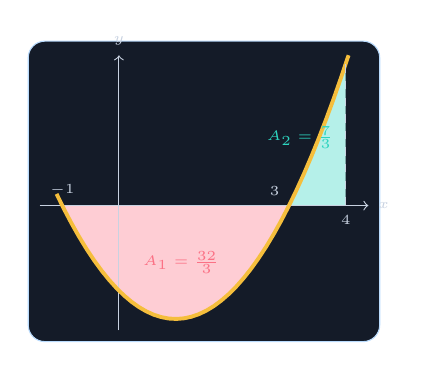
\begin{tikzpicture}[xscale=0.72, yscale=0.36]
                \draw[fill=DarkBox, draw=ElectricBlue!40, rounded corners=6pt] (-1.6,-4.8) rectangle (4.6,5.8);
                \fill[color=CoralRose!35, domain=-1:3, samples=30]
                    (-1,0) -- plot (\x, {\x*\x - 2*\x - 3}) -- (3,0) -- cycle;
                \fill[color=TealCyan!35, domain=3:4, samples=20]
                    (3,0) -- plot (\x, {\x*\x - 2*\x - 3}) -- (4,0) -- cycle;
                \draw[->, color=SoftGray] (-1.4,0) -- (4.4,0) node[right] {\tiny $x$};
                \draw[->, color=SoftGray] (0,-4.4) -- (0,5.3) node[above] {\tiny $y$};
                \draw[color=LuminousGold, line width=1.4pt, domain=-1.1:4.05, samples=40]
                    plot (\x, {\x*\x - 2*\x - 3});
                \draw[dashed, color=SoftGray] (4,0) -- (4,5);
                \node[above, color=SoftGray] at (-1,0) {\tiny $-1$};
                \node[above left, color=SoftGray] at (3,0) {\tiny $3$};
                \node[below, color=SoftGray] at (4,0) {\tiny $4$};
                \node[color=CoralRose] at (1.1,-2.0) {\tiny $A_1 = \frac{32}{3}$};
                \node[color=TealCyan] at (3.2,2.4) {\tiny $A_2 = \frac{7}{3}$};
            \end{tikzpicture}
            \vskip 2pt
            {\tiny\color{CoralRose}Hati-hati: $\int_{-1}^4 f(x)\,dx = -\frac{32}{3} + \frac{7}{3} = -\frac{25}{3} \neq 13$!}
        \end{column}
    \end{columns}
\end{frame}

% -------------------------------------------------------------
% Slide 5: Luas Daerah di Antara Dua Kurva (Pias Tegak Δx)
% -------------------------------------------------------------
\begin{frame}{Luas Daerah di Antara Dua Kurva dengan Pias Tegak ($\Delta x$)}
    \begin{columns}[c]
        \begin{column}{0.54\textwidth}
            \begin{block}{Penurunan Rumus Pias Tegak ($\Delta x$)}
                \scriptsize\abovedisplayskip=3pt\belowdisplayskip=3pt
                Misalkan $y = f(x)$ dan $y = g(x)$ kontinu pada $[a, b]$ dengan $\mathbf{f(x) \ge g(x)}$ untuk setiap $x \in [a, b]$:
                \begin{itemize}\itemsep=2pt
                    \item Iris daerah secara vertikal dengan pias selebar $\Delta x$.
                    \item Tinggi pias pada posisi $x$ adalah jarak vertikal dari kurva bawah ke kurva atas:
                    $$h(x) = y_{\text{atas}} - y_{\text{bawah}} = f(x) - g(x) \ge 0.$$
                    \item Elemen luas $\Delta A \approx [f(x) - g(x)]\,\Delta x$ menghasilkan:
                \end{itemize}
                $$\boxed{A = \int_{a}^{b} \big(y_{\text{atas}} - y_{\text{bawah}}\big)\,dx = \int_{a}^{b} \big[f(x) - g(x)\big]\,dx}$$
            \end{block}

            \begin{alertblock}{Mengapa Tetap Berlaku Saat $g(x) < 0$?}
                \scriptsize
                Jika $g(x) < 0$, jarak dari sumbu-$x$ ke kurva bawah adalah $-g(x) > 0$. Maka tinggi total pias adalah $f(x) + \big(-g(x)\big) = \mathbf{f(x) - g(x)}$! Rumus tidak berubah di mana pun letak sumbu-$x$.
            \end{alertblock}
        \end{column}

        \begin{column}{0.43\textwidth}
            \centering
            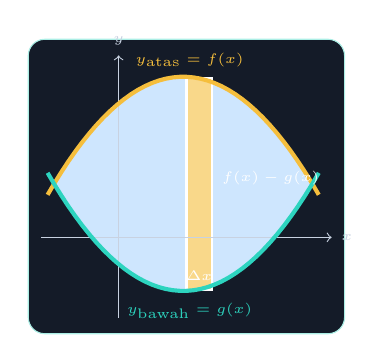
\begin{tikzpicture}[xscale=0.82, yscale=0.68]
                \draw[fill=DarkBox, draw=TealCyan!40, rounded corners=6pt] (-1.4,-1.8) rectangle (3.5,3.7);
                \fill[color=ElectricBlue!28, domain=-1:3, samples=40]
                    plot (\x, {3 - 0.5*(\x-1)*(\x-1)}) --
                    plot[domain=3:-1, samples=40] (\x, {0.5*(\x-1)*(\x-1) - 1}) -- cycle;
                % Pias tegak di x = 1.2
                \fill[color=LuminousGold!60, draw=white, line width=0.8pt]
                    (1.05, -0.98) rectangle (1.45, 2.98);
                \draw[->, color=SoftGray] (-1.2,0) -- (3.3,0) node[right] {\tiny $x$};
                \draw[->, color=SoftGray] (0,-1.5) -- (0,3.4) node[above] {\tiny $y$};
                \draw[color=LuminousGold, line width=1.5pt, domain=-1.1:3.1, samples=40]
                    plot (\x, {3 - 0.5*(\x-1)*(\x-1)});
                \draw[color=TealCyan, line width=1.5pt, domain=-1.1:3.1, samples=40]
                    plot (\x, {0.5*(\x-1)*(\x-1) - 1});
                \node[above, color=LuminousGold] at (1.1,3.0) {\tiny $y_{\text{atas}} = f(x)$};
                \node[below, color=TealCyan] at (1.1,-1.05) {\tiny $y_{\text{bawah}} = g(x)$};
                \node[right, color=white] at (1.45, 1.1) {\tiny $f(x)-g(x)$};
                \node[above, color=white] at (1.25, -0.98) {\tiny $\Delta x$};
            \end{tikzpicture}
        \end{column}
    \end{columns}
\end{frame}

% -------------------------------------------------------------
% Slide 6: Simulasi Video 1 - AreaBetweenCurvesVerticalScene
% -------------------------------------------------------------
\begin{frame}{Simulasi Dinamis: Pias Tegak ($\Delta x$) di Antara Dua Kurva}
    \centering
    \movie[width=0.66\textwidth,height=0.44\textwidth,poster,showcontrols=true]%
        {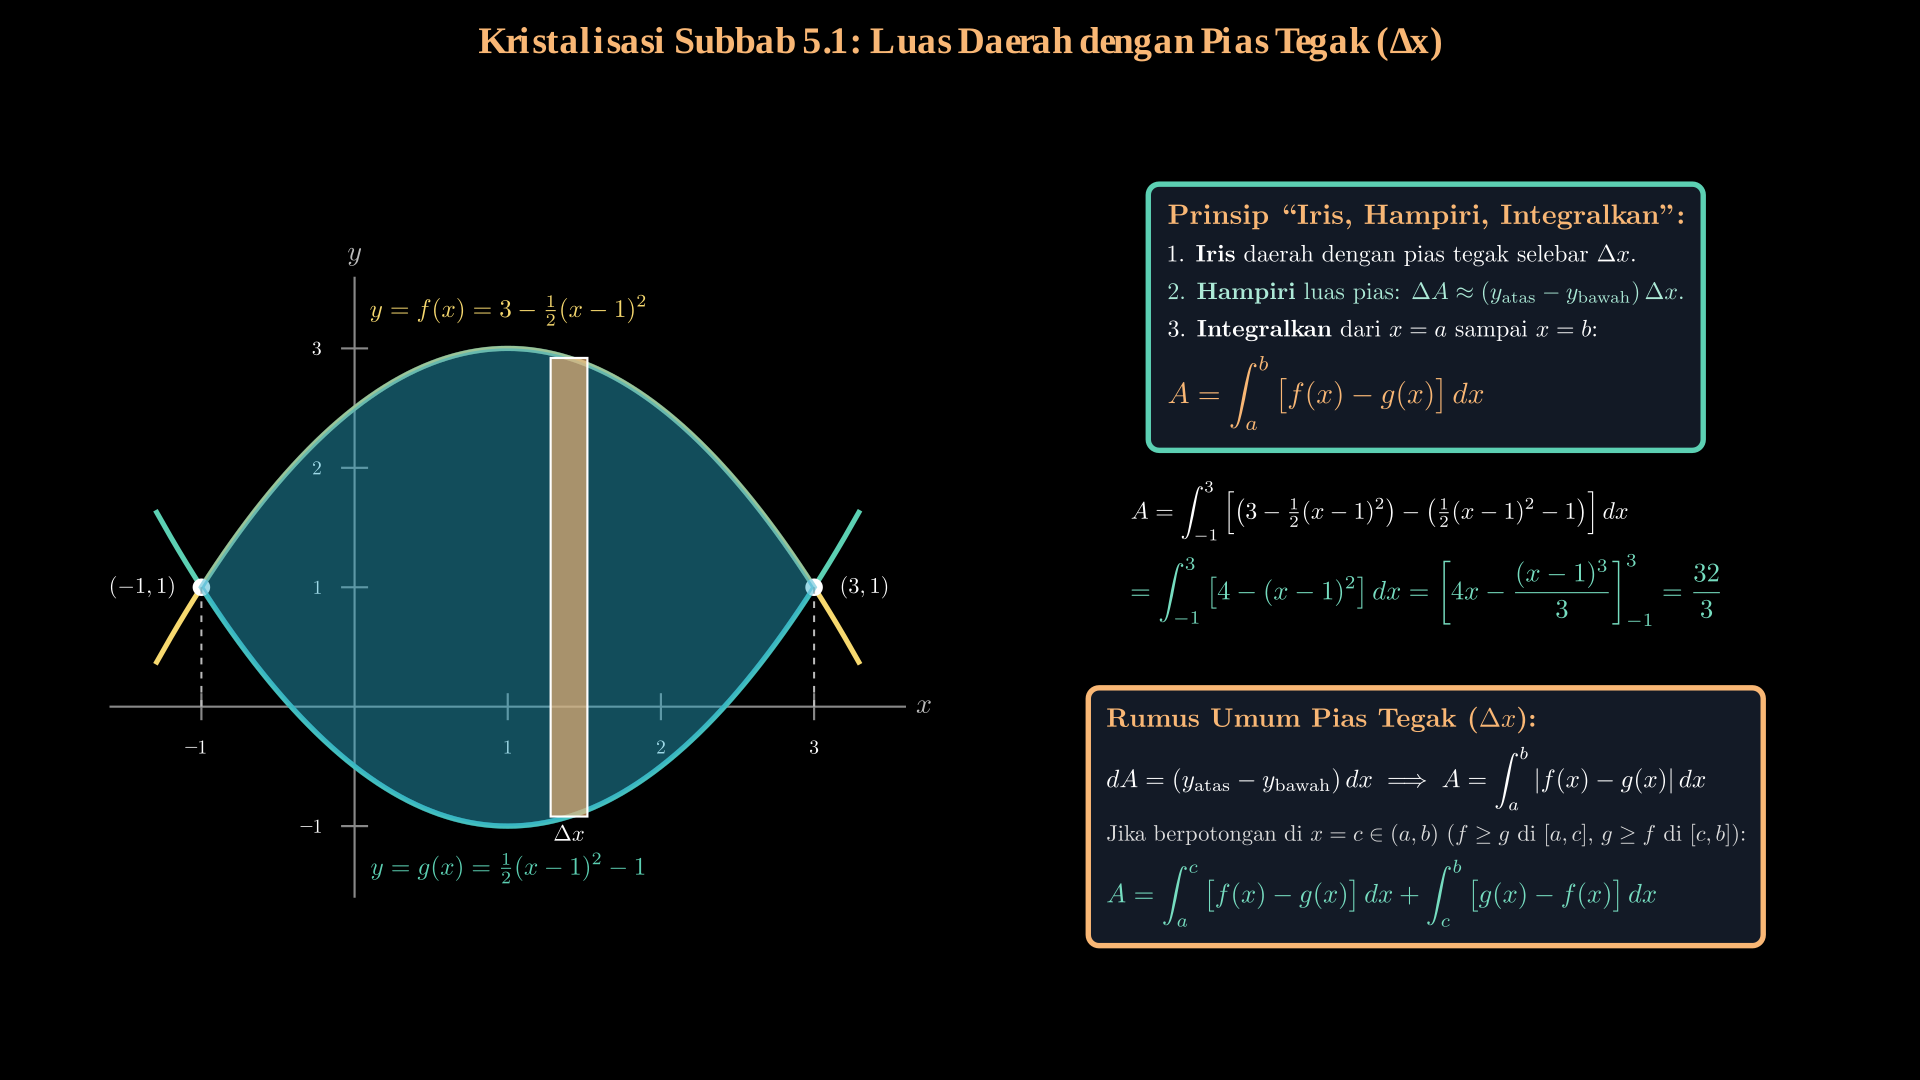
\includegraphics[width=0.66\textwidth,height=0.44\textwidth]{keyframe_luas_pias_tegak.png}}%
        {AreaBetweenCurvesVerticalScene.ogv}

    \vskip 0.2em
    \href{run:./play_video.sh tegak}{%
        \beamerbutton{\small\color{white} $\blacktriangleright$ Putar Video Animasi (\texttt{AreaBetweenCurvesVerticalScene.mp4})}%
    }

    \vskip 0.2em
    \tiny\textit{\color{SoftGray}Klik poster untuk pemutaran langsung di Pympress/Okular, atau klik tombol untuk memutar di MPV/VLC.}
\end{frame}

% -------------------------------------------------------------
% Slide 7: Contoh 2 - Luas di Antara Dua Kurva (Menentukan Titik Potong)
% -------------------------------------------------------------
\begin{frame}{Contoh 2: Daerah yang Dibatasi oleh Dua Parabola}
    \begin{exampleblock}{Soal}
        \scriptsize
        Tentukan luas daerah yang dibatasi oleh kurva $y = 4 - x^2$ dan $y = x^2 - 2x$! (Perhatikan bahwa batas kiri $a$ dan batas kanan $b$ tidak diberikan secara eksplisit).
    \end{exampleblock}

    \begin{columns}[T]
        \begin{column}{0.48\textwidth}
            \begin{block}{1. Cari Titik Potong ($f(x) = g(x)$)}
                \scriptsize\abovedisplayskip=2pt\belowdisplayskip=2pt
                Samakan kedua persamaan kurva untuk memperoleh batas integrasi:
                \begin{align*}
                    4 - x^2 &= x^2 - 2x\\
                    2x^2 - 2x - 4 &= 0\\
                    2(x + 1)(x - 2) &= 0 \implies \mathbf{x = -1} \;\text{dan}\; \mathbf{x = 2}.
                \end{align*}
                Pada $[-1, 2]$, uji di $x = 0$: kurva $y = 4 - x^2$ bernilai $4$, sedangkan $y = x^2 - 2x$ bernilai $0$. Jadi:
                $$y_{\text{atas}} = 4 - x^2, \qquad y_{\text{bawah}} = x^2 - 2x.$$
            \end{block}
        \end{column}

        \begin{column}{0.48\textwidth}
            \begin{alertblock}{2. Iris, Hampiri, Integralkan}
                \scriptsize\abovedisplayskip=2pt\belowdisplayskip=2pt
                Tinggi pias tegak adalah:
                $$y_{\text{atas}} - y_{\text{bawah}} = (4 - x^2) - (x^2 - 2x) = 4 + 2x - 2x^2.$$
                Maka luas daerahnya:
                \begin{align*}
                    A &= \int_{-1}^{2} (4 + 2x - 2x^2)\,dx\\
                    &= \left[4x + x^2 - \frac{2}{3}x^3\right]_{-1}^{2}\\
                    &= \left(8 + 4 - \frac{16}{3}\right) - \left(-4 + 1 + \frac{2}{3}\right) = \mathbf{9}.
                \end{align*}
            \end{alertblock}
        \end{column}
    \end{columns}
\end{frame}

% -------------------------------------------------------------
% Slide 8: Dua Kurva yang Saling Berpotongan (Berganti Atas-Bawah)
% -------------------------------------------------------------
\begin{frame}{Daerah dengan Dua Kurva yang Saling Berpotongan}
    \begin{block}{Bagaimana Jika $f(x)$ dan $g(x)$ Bertukar Posisi Atas-Bawah?}
        \scriptsize\abovedisplayskip=3pt\belowdisplayskip=3pt
        Jika kurva $y = f(x)$ dan $y = g(x)$ berpotongan di satu atau lebih titik di dalam selang $(a, b)$, maka selisih $f(x) - g(x)$ akan \textbf{berganti tanda}. Agar tinggi pias selalu positif, tinggi pias pada sebarang titik $x$ adalah $\mathbf{|f(x) - g(x)|}$:
        $$\boxed{\;A = \int_{a}^{b} \big|f(x) - g(x)\big|\,dx\;}$$
    \end{block}

    \begin{columns}[T]
        \begin{column}{0.48\textwidth}
            \begin{exampleblock}{Prosedur Baku (3 Langkah)}
                \scriptsize
                \begin{enumerate}\itemsep=2pt
                    \item Selesaikan persamaan $\mathbf{f(x) = g(x)}$ untuk menemukan semua titik potong $c_1, c_2, \dots$ yang jatuh di dalam $(a, b)$.
                    \item Pecah integral pada setiap titik potong tersebut.
                    \item Pada tiap subselang, integralkan $\mathbf{(y_{\text{atas}} - y_{\text{bawah}})\,dx}$.
                \end{enumerate}
            \end{exampleblock}
        \end{column}

        \begin{column}{0.48\textwidth}
            \begin{alertblock}{Jika Berpotongan di Satu Titik $c \in (a,b)$}
                \scriptsize\abovedisplayskip=2pt\belowdisplayskip=2pt
                Misalkan $f(x) \ge g(x)$ pada $[a, c]$ dan $g(x) \ge f(x)$ pada $[c, b]$, maka:
                \begin{align*}
                    A &= \int_{a}^{c} \big[f(x) - g(x)\big]\,dx\\
                    &\quad + \int_{c}^{b} \big[g(x) - f(x)\big]\,dx.
                \end{align*}
            \end{alertblock}
        \end{column}
    \end{columns}
\end{frame}

% -------------------------------------------------------------
% Slide 9: Contoh 3 - Dua Kurva Berpotongan di Tiga Titik
% -------------------------------------------------------------
\begin{frame}{Contoh 3: Kurva Kubik dan Garis yang Berpotongan di 3 Titik}
    \begin{exampleblock}{Soal}
        \scriptsize
        Tentukan luas daerah yang dibatasi oleh kurva $y = x^3 - 3x$ dan garis $y = x$!
    \end{exampleblock}

    \begin{columns}[c]
        \begin{column}{0.55\textwidth}
            \begin{block}{Penyelesaian}
                \scriptsize\abovedisplayskip=2pt\belowdisplayskip=2pt
                \begin{enumerate}\itemsep=1pt
                    \item \textbf{Titik potong}: $x^3 - 3x = x \iff x(x - 2)(x + 2) = 0 \implies \mathbf{x = -2, \;0, \;2}$.
                    \item \textbf{Posisi kurva}:
                    \begin{itemize}\scriptsize\itemsep=0pt
                        \item Pada $[-2, 0]$: kubik di atas $\implies y_{\text{atas}} - y_{\text{bawah}} = x^3 - 4x$.
                        \item Pada $[0, 2]$: garis di atas $\implies y_{\text{atas}} - y_{\text{bawah}} = 4x - x^3$.
                    \end{itemize}
                    \item \textbf{Integralkan} (atau gunakan simetri fungsi genap $|x^3 - 4x|$!):
                    \begin{align*}
                        A &= \int_{-2}^{0} (x^3 - 4x)\,dx + \int_{0}^{2} (4x - x^3)\,dx\\
                        &= 2\int_{0}^{2} (4x - x^3)\,dx = 2\left[2x^2 - \frac{x^4}{4}\right]_{0}^{2} = \mathbf{8}.
                    \end{align*}
                \end{enumerate}
            \end{block}
        \end{column}

        \begin{column}{0.41\textwidth}
            \centering
            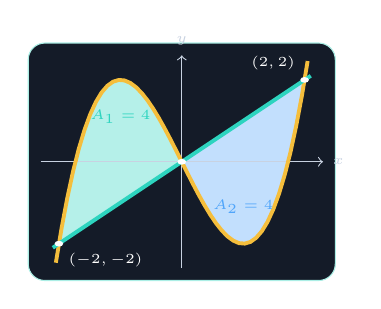
\begin{tikzpicture}[xscale=0.78, yscale=0.52]
                \draw[fill=DarkBox, draw=TealCyan!40, rounded corners=6pt] (-2.5,-2.9) rectangle (2.5,2.9);
                \fill[color=TealCyan!35, domain=-2:0, samples=30]
                    plot (\x, {\x*\x*\x - 3*\x}) -- (0,0) -- (-2,-2) -- cycle;
                \fill[color=ElectricBlue!35, domain=0:2, samples=30]
                    (0,0) -- (2,2) -- plot[domain=2:0, samples=30] (\x, {\x*\x*\x - 3*\x}) -- cycle;
                \draw[->, color=SoftGray] (-2.3,0) -- (2.3,0) node[right] {\tiny $x$};
                \draw[->, color=SoftGray] (0,-2.6) -- (0,2.6) node[above] {\tiny $y$};
                \draw[color=LuminousGold, line width=1.4pt, domain=-2.05:2.05, samples=45]
                    plot (\x, {\x*\x*\x - 3*\x});
                \draw[color=TealCyan, line width=1.4pt] (-2.1,-2.1) -- (2.1,2.1);
                \fill[color=white] (-2,-2) circle (2pt) node[below right] {\tiny $(-2,-2)$};
                \fill[color=white] (0,0) circle (2pt);
                \fill[color=white] (2,2) circle (2pt) node[above left] {\tiny $(2,2)$};
                \node[color=TealCyan] at (-1.0,1.1) {\tiny $A_1=4$};
                \node[color=ElectricBlue] at (1.0,-1.1) {\tiny $A_2=4$};
            \end{tikzpicture}
        \end{column}
    \end{columns}
\end{frame}

% -------------------------------------------------------------
% Slide 10: Contoh 4 - Kurva Trigonometri yang Berpotongan
% -------------------------------------------------------------
\begin{frame}{Contoh 4: Daerah di Antara $\sin x$ dan $\cos x$ pada $[0, \pi]$}
    \begin{exampleblock}{Soal}
        \scriptsize
        Hitunglah luas daerah yang dibatasi oleh kurva $y = \sin x$ dan $y = \cos x$ pada selang $[0, \pi]$!
    \end{exampleblock}

    \begin{columns}[c]
        \begin{column}{0.55\textwidth}
            \begin{block}{Penyelesaian}
                \scriptsize\abovedisplayskip=2pt\belowdisplayskip=2pt
                \begin{enumerate}\itemsep=1pt
                    \item Cari titik potong pada $[0, \pi]$:
                    $$\sin x = \cos x \iff \tan x = 1 \implies \mathbf{x = \frac{\pi}{4}}.$$
                    \item Periksa siapa yang berada di atas:
                    \begin{itemize}\scriptsize\itemsep=0pt
                        \item Pada $\left[0, \frac{\pi}{4}\right]$: $\cos x \ge \sin x$.
                        \item Pada $\left[\frac{\pi}{4}, \pi\right]$: $\sin x \ge \cos x$ (perhatikan bahwa pada $\left[\frac{\pi}{2}, \pi\right]$, $\cos x \le 0$!).
                    \end{itemize}
                    \item Maka luas totalnya adalah:
                    \begin{align*}
                        A &= \int_{0}^{\pi/4} (\cos x - \sin x)\,dx + \int_{\pi/4}^{\pi} (\sin x - \cos x)\,dx\\
                        &= \big[\sin x + \cos x\big]_{0}^{\pi/4} + \big[-\cos x - \sin x\big]_{\pi/4}^{\pi}\\
                        &= \big(\sqrt{2} - 1\big) + \big(1 - (-\sqrt{2})\big) = \mathbf{2\sqrt{2}}.
                    \end{align*}
                \end{enumerate}
            \end{block}
        \end{column}

        \begin{column}{0.41\textwidth}
            \centering
            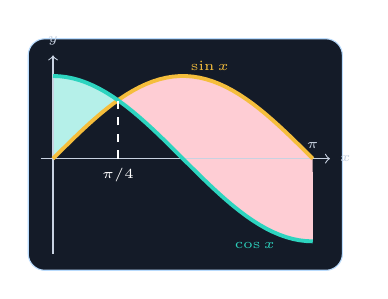
\begin{tikzpicture}[xscale=1.05, yscale=1.05]
                \draw[fill=DarkBox, draw=ElectricBlue!40, rounded corners=6pt] (-0.3,-1.35) rectangle (3.5,1.45);
                \fill[color=TealCyan!35, domain=0:0.7854, samples=20]
                    plot (\x, {cos(\x r)}) -- plot[domain=0.7854:0, samples=20] (\x, {sin(\x r)}) -- cycle;
                \fill[color=CoralRose!35, domain=0.7854:3.1416, samples=35]
                    plot (\x, {sin(\x r)}) -- plot[domain=3.1416:0.7854, samples=35] (\x, {cos(\x r)}) -- cycle;
                \draw[->, color=SoftGray] (-0.15,0) -- (3.35,0) node[right] {\tiny $x$};
                \draw[->, color=SoftGray] (0,-1.15) -- (0,1.25) node[above] {\tiny $y$};
                \draw[color=LuminousGold, line width=1.4pt, domain=0:3.1416, samples=40]
                    plot (\x, {sin(\x r)});
                \draw[color=TealCyan, line width=1.4pt, domain=0:3.1416, samples=40]
                    plot (\x, {cos(\x r)});
                \draw[dashed, color=white] (0.7854,0) -- (0.7854,0.7071);
                \node[below, color=white] at (0.7854,0) {\tiny $\pi/4$};
                \node[above, color=SoftGray] at (3.14,0) {\tiny $\pi$};
                \node[above right, color=LuminousGold] at (1.55,0.95) {\tiny $\sin x$};
                \node[below left, color=TealCyan] at (2.8,-0.9) {\tiny $\cos x$};
            \end{tikzpicture}
        \end{column}
    \end{columns}
\end{frame}

% -------------------------------------------------------------
% Slide 11: Pengantar Pias Mendatar (Δy / Horizontal Slicing)
% -------------------------------------------------------------
\begin{frame}{Pengantar Pias Mendatar ($\Delta y$ / \textit{Horizontal Slicing})}
    \begin{columns}[c]
        \begin{column}{0.54\textwidth}
            \begin{block}{Kapan Kita Memutar Pias Menjadi Mendatar ($\Delta y$)?}
                \scriptsize\abovedisplayskip=3pt\belowdisplayskip=3pt
                Terkadang kurva pembatas lebih mudah dinyatakan sebagai fungsi dari $y$, yaitu $\mathbf{x = p(y)}$ (batas kanan) dan $\mathbf{x = q(y)}$ (batas kiri) untuk $y \in [c, d]$ dengan $p(y) \ge q(y)$:
                \begin{itemize}\itemsep=2pt
                    \item Iris daerah secara \textbf{mendatar (horizontal)} dengan pias setebal $\mathbf{\Delta y}$.
                    \item Panjang mendatar pias pada ketinggian $y$ adalah:
                    $$\text{panjang} = x_{\text{kanan}} - x_{\text{kiri}} = p(y) - q(y) \ge 0.$$
                    \item Elemen luas $\Delta A \approx [p(y) - q(y)]\,\Delta y$ menghasilkan:
                \end{itemize}
                $$\boxed{A = \int_{c}^{d} \big(x_{\text{kanan}} - x_{\text{kiri}}\big)\,dy = \int_{c}^{d} \big[p(y) - q(y)\big]\,dy}$$
            \end{block}
        \end{column}

        \begin{column}{0.43\textwidth}
            \centering
            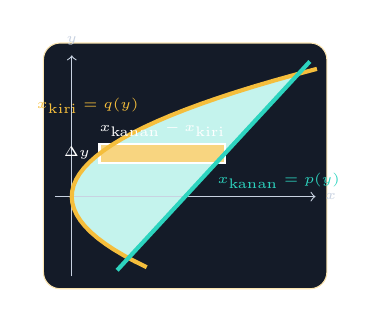
\begin{tikzpicture}[xscale=0.72, yscale=0.78]
                \draw[fill=DarkBox, draw=LuminousGold!40, rounded corners=6pt] (-0.5,-1.5) rectangle (4.5,2.5);
                \fill[color=TealCyan!28]
                    plot[domain=-1:2, samples=30] ({\x*\x}, \x) --
                    plot[domain=2:-1, samples=30] ({\x+2}, \x) -- cycle;
                % Pias mendatar di y = 0.7
                \fill[color=LuminousGold!65, draw=white, line width=0.8pt]
                    (0.49, 0.55) rectangle (2.7, 0.85);
                \draw[->, color=SoftGray] (-0.3,0) -- (4.3,0) node[right] {\tiny $x$};
                \draw[->, color=SoftGray] (0,-1.3) -- (0,2.3) node[above] {\tiny $y$};
                \draw[color=LuminousGold, line width=1.5pt, domain=-1.15:2.08, samples=35]
                    plot ({\x*\x}, \x);
                \draw[color=TealCyan, line width=1.5pt] (0.8,-1.2) -- (4.2,2.2);
                \node[left, color=LuminousGold] at (1.35, 1.48) {\tiny $x_{\text{kiri}}=q(y)$};
                \node[right, color=TealCyan] at (2.4, 0.25) {\tiny $x_{\text{kanan}}=p(y)$};
                \node[above, color=white] at (1.6, 0.82) {\tiny $x_{\text{kanan}}-x_{\text{kiri}}$};
                \node[left, color=white] at (0.49, 0.7) {\tiny $\Delta y$};
            \end{tikzpicture}
        \end{column}
    \end{columns}
\end{frame}

% -------------------------------------------------------------
% Slide 12: Simulasi Video 2 - AreaHorizontalVsVerticalScene
% -------------------------------------------------------------
\begin{frame}{Simulasi Dinamis: Pias Mendatar ($\Delta y$) vs.\ Pias Tegak ($\Delta x$)}
    \centering
    \movie[width=0.66\textwidth,height=0.44\textwidth,poster,showcontrols=true]%
        {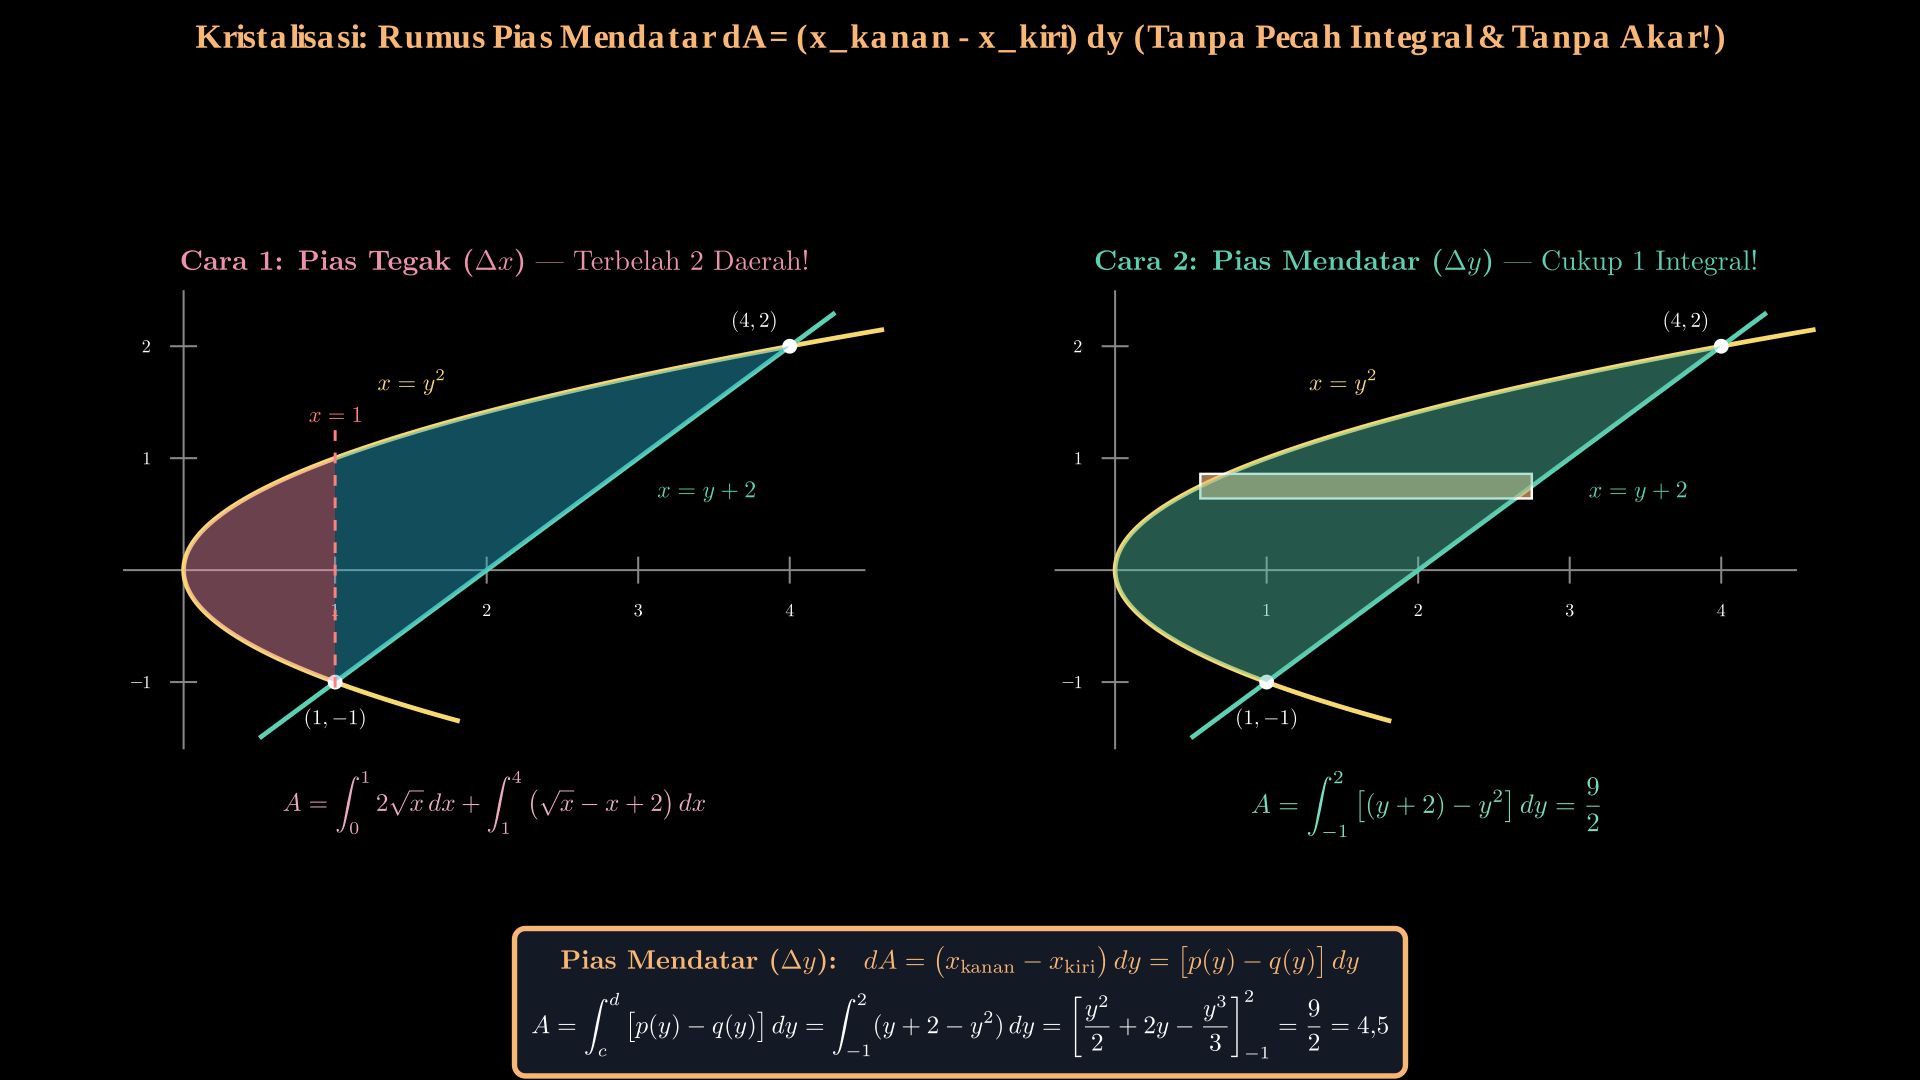
\includegraphics[width=0.66\textwidth,height=0.44\textwidth]{keyframe_luas_pias_mendatar.png}}%
        {AreaHorizontalVsVerticalScene.ogv}

    \vskip 0.2em
    \href{run:./play_video.sh mendatar}{%
        \beamerbutton{\small\color{white} $\blacktriangleright$ Putar Video Animasi (\texttt{AreaHorizontalVsVerticalScene.mp4})}%
    }

    \vskip 0.2em
    \tiny\textit{\color{SoftGray}Bandingkan bagaimana pias tegak ($\Delta x$) terbelah di $x=1$, sedangkan pias mendatar ($\Delta y$) menyapu mulus dengan 1 integral!}
\end{frame}

% -------------------------------------------------------------
% Slide 13: Contoh 5 - Perbandingan Langsung Δy vs Δx pada Daerah yang Sama
% -------------------------------------------------------------
\begin{frame}{Contoh 5: Menghitung Luas Daerah $y^2 = 4x$ dan $4x - 3y = 4$}
    \begin{exampleblock}{Soal (Purcell \S5.1)}
        \scriptsize
        Tentukan luas daerah $R$ yang dibatasi oleh parabola $y^2 = 4x$ dan garis $4x - 3y = 4$ dengan \textbf{(a) Pias Mendatar ($\Delta y$)} dan \textbf{(b) Pias Tegak ($\Delta x$)}!
    \end{exampleblock}

    \begin{columns}[T]
        \begin{column}{0.48\textwidth}
            \begin{block}{(a) Dengan Pias Mendatar ($\Delta y$) --- SANGAT MUDAH}
                \scriptsize\abovedisplayskip=2pt\belowdisplayskip=2pt
                Nyatakan $x$ sebagai fungsi dari $y$:
                $$x_{\text{kiri}} = \frac{y^2}{4}, \qquad x_{\text{kanan}} = \frac{3y + 4}{4}.$$
                Titik potong: $y^2 = 3y + 4 \iff (y - 4)(y + 1) = 0 \implies \mathbf{y = -1}$ dan $\mathbf{y = 4}$ (yakni titik $\left(\frac{1}{4}, -1\right)$ dan $(4, 4)$).\\
                Maka cukup \textbf{1 integral polinom}:
                \begin{align*}
                    A &= \int_{-1}^{4} \left(\frac{3y + 4}{4} - \frac{y^2}{4}\right)dy\\
                    &= \frac{1}{4}\left[\frac{3y^2}{2} + 4y - \frac{y^3}{3}\right]_{-1}^{4} = \mathbf{\frac{125}{24} \approx 5{,}21}.
                \end{align*}
            \end{block}
        \end{column}

        \begin{column}{0.48\textwidth}
            \begin{alertblock}{(b) Dengan Pias Tegak ($\Delta x$) --- HARUS PECAH 2!}
                \scriptsize\abovedisplayskip=2pt\belowdisplayskip=2pt
                Jika dipaksa memakai $\Delta x$, kita harus menulis $y = \pm 2\sqrt{x}$ dan $y = \frac{4x - 4}{3}$:
                \begin{itemize}\itemsep=1pt
                    \item Pada $\left[0, \frac{1}{4}\right]$: batas atas $y = 2\sqrt{x}$, batas bawah $y = -2\sqrt{x}$.
                    \item Pada $\left[\frac{1}{4}, 4\right]$: batas atas $y = 2\sqrt{x}$, batas bawah berganti menjadi garis $y = \frac{4x - 4}{3}$!
                \end{itemize}
                $$A = \int_{0}^{1/4}\! 4\sqrt{x}\,dx + \int_{1/4}^{4}\! \big(2\sqrt{x} - \tfrac{4x - 4}{3}\big)\,dx = \mathbf{\frac{125}{24}}.$$
                {\tiny\color{TealCyan}Kedua cara menghasilkan nilai yang sama persis, tetapi $\Delta y$ jauh lebih hemat waktu!}
            \end{alertblock}
        \end{column}
    \end{columns}
\end{frame}

% -------------------------------------------------------------
% Slide 14: Contoh 6 - Daerah yang Dibatasi Tiga Kurva (Segitiga Melengkung)
% -------------------------------------------------------------
\begin{frame}{Contoh 6: Daerah yang Dibatasi oleh Tiga Kurva}
    \begin{exampleblock}{Soal}
        \scriptsize
        Tentukan luas daerah $R$ di kuadran pertama yang dibatasi oleh kurva $y = x^2$, garis $y = 2 - x$, dan sumbu-$x$ ($y = 0$)!
    \end{exampleblock}

    \begin{columns}[c]
        \begin{column}{0.56\textwidth}
            \begin{block}{Bandingkan $\Delta x$ (2 Integral) vs.\ $\Delta y$ (1 Integral)}
                \scriptsize\abovedisplayskip=2pt\belowdisplayskip=2pt
                Titik potong $y = x^2$ dan $y = 2 - x$ di kuadran I:
                $$x^2 = 2 - x \iff (x + 2)(x - 1) = 0 \implies \mathbf{(1, 1)}.$$
                \begin{itemize}\itemsep=2pt
                    \item \textbf{Cara 1 (Pias Tegak $\Delta x$)}: Batas atas berganti di $x = 1$!
                    $$A = \int_{0}^{1} x^2\,dx + \int_{1}^{2} (2 - x)\,dx = \frac{1}{3} + \frac{1}{2} = \mathbf{\frac{5}{6}}.$$
                    \item \textbf{Cara 2 (Pias Mendatar $\Delta y$)}: Untuk $y \in [0, 1]$, batas kanan selalu garis $x_{\text{kanan}} = 2 - y$ dan batas kiri selalu parabola $x_{\text{kiri}} = \sqrt{y}$:
                    $$A = \int_{0}^{1} \!\big(2 - y - \sqrt{y}\big)\,dy = \left[2y - \frac{y^2}{2} - \frac{2}{3}y^{3/2}\right]_{0}^{1}\! = \mathbf{\frac{5}{6}}.$$
                \end{itemize}
            \end{block}
        \end{column}

        \begin{column}{0.40\textwidth}
            \centering
            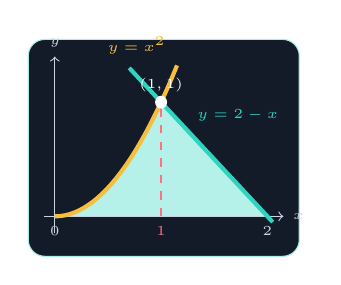
\begin{tikzpicture}[xscale=1.35, yscale=1.45]
                \draw[fill=DarkBox, draw=TealCyan!40, rounded corners=6pt] (-0.25,-0.35) rectangle (2.3,1.55);
                \fill[color=TealCyan!35, domain=0:1, samples=25]
                    (0,0) -- plot (\x, {\x*\x}) -- (1,1) -- (2,0) -- cycle;
                \draw[->, color=SoftGray] (-0.1,0) -- (2.15,0) node[right] {\tiny $x$};
                \draw[->, color=SoftGray] (0,-0.15) -- (0,1.4) node[above] {\tiny $y$};
                \draw[color=LuminousGold, line width=1.5pt, domain=0:1.15, samples=25]
                    plot (\x, {\x*\x}) node[above left] {\tiny $y=x^2$};
                \draw[color=TealCyan, line width=1.5pt] (0.7,1.3) -- (2.05,-0.05);
                \node[above right, color=TealCyan] at (1.25,0.75) {\tiny $y=2-x$};
                \draw[dashed, color=CoralRose, thick] (1,0) -- (1,1);
                \fill[color=white] (1,1) circle (1.6pt) node[above] {\tiny $(1,1)$};
                \node[below, color=SoftGray] at (0,0) {\tiny $0$};
                \node[below, color=CoralRose] at (1,0) {\tiny $1$};
                \node[below, color=SoftGray] at (2,0) {\tiny $2$};
            \end{tikzpicture}
        \end{column}
    \end{columns}
\end{frame}

% -------------------------------------------------------------
% Slide 15: Panduan Strategis Memilih Pias Tegak (Δx) vs Mendatar (Δy)
% -------------------------------------------------------------
\begin{frame}{Panduan Strategis: Kapan Memilih $\Delta x$ vs.\ $\Delta y$?}
    \begin{block}{Tabel Perbandingan Pias Tegak ($\Delta x$) dan Pias Mendatar ($\Delta y$)}
        \scriptsize
        \renewcommand{\arraystretch}{1.45}
        \centering
        \begin{tabular}{@{}p{0.22\textwidth}p{0.35\textwidth}p{0.35\textwidth}@{}}
            \textbf{Aspek} & \textbf{Pias Tegak ($\Delta x$ / Vertikal)} & \textbf{Pias Mendatar ($\Delta y$ / Horizontal)}\\\hline
            \textbf{Persamaan Kurva} & Eksplisit dalam $x$: $y = f(x)$ dan $y = g(x)$ & Eksplisit dalam $y$: $x = p(y)$ dan $x = q(y)$\\
            \textbf{Ukuran Pias} & Lebar $= \Delta x$, Tinggi $= y_{\text{atas}} - y_{\text{bawah}}$ & Tebal $= \Delta y$, Panjang $= x_{\text{kanan}} - x_{\text{kiri}}$\\
            \textbf{Elemen Luas $dA$} & $dA = \big[f(x) - g(x)\big]\,dx$ & $dA = \big[p(y) - q(y)\big]\,dy$\\
            \textbf{Batas Integrasi} & Absis ekstrem kiri $x = a$ s.d.\ kanan $x = b$ & Ordinat ekstrem bawah $y = c$ s.d.\ atas $y = d$\\
            \textbf{Kapan Terbaik?} & Batas atas \& bawah tidak berganti rumus sepanjang $[a, b]$ & Kurva berupa $x = y^2, x = y^3$, atau batas kiri-kanan tunggal sepanjang $[c, d]$\\
        \end{tabular}
    \end{block}

    \begin{alertblock}{Tips Emas di Ujian MA1101}
        \scriptsize
        Selalu \textbf{gambar sketsa kasar daerah terlebih dahulu} dan tarik satu garis uji vertikal serta satu garis uji horizontal! Pilih arah pias yang \textbf{tidak mengalami pergantian kurva batas} (sehingga cukup 1 integral) dan \textbf{menghindari bentuk akar/invers yang sulit diintegralkan}.
    \end{alertblock}
\end{frame}

% -------------------------------------------------------------
% Slide 16: Tafsiran Fisika — Luas di Antara Dua Kurva Kecepatan
% -------------------------------------------------------------
\begin{frame}{Aplikasi Fisika: Luas di Antara Dua Kurva Kecepatan}
    \begin{block}{Tafsiran Fisis $\int_{t_1}^{t_2} [v_A(t) - v_B(t)]\,dt$}
        \scriptsize
        Jika dua benda $A$ dan $B$ bergerak sepanjang lintasan lurus dengan kecepatan masing-masing $v_A(t)$ dan $v_B(t)$ (dengan $v_A(t) \ge v_B(t)$ pada $[0, T]$), maka \textbf{luas daerah di antara kedua kurva kecepatan} menyatakan \textbf{selisih jarak tempuh} antara benda $A$ dan benda $B$:
        $$A = \int_{0}^{T} \big[v_A(t) - v_B(t)\big]\,dt = \int_{0}^{T} v_A(t)\,dt - \int_{0}^{T} v_B(t)\,dt = s_A(T) - s_B(T).$$
    \end{block}

    \begin{exampleblock}{Contoh Kinematika: Kapan Pelari Kedua Menyusul Pelari Pertama?}
        \scriptsize\abovedisplayskip=2pt\belowdisplayskip=2pt
        Dua pelari berangkat dari garis \textit{start} yang sama pada $t = 0$. Pelari $A$ berlari dengan kecepatan konstan $v_A(t) = 6\text{ m/s}$, sedangkan pelari $B$ mempercepat larinya menurut $v_B(t) = 2t\text{ m/s}$.
        \begin{itemize}\itemsep=1pt
            \item Pada $t \in [0, 3]$, $v_A(t) > v_B(t)$: luas segitiga di antara kedua kurva adalah jarak keunggulan maksimum pelari $A$ pada $t = 3\text{ s}$, yaitu $\int_0^3 (6 - 2t)\,dt = \mathbf{9\text{ meter}}$.
            \item Pelari $B$ menyusul pelari $A$ pada waktu $T > 3$ ketika luas di mana $v_B > v_A$ pada $[3, T]$ tepat menyamai $9\text{ m}$:
            $$\int_{3}^{T} (2t - 6)\,dt = (T - 3)^2 = 9 \implies T - 3 = 3 \implies \mathbf{T = 6\text{ detik}}.$$
        \end{itemize}
    \end{exampleblock}
\end{frame}

% -------------------------------------------------------------
% Slide 17: Soal Tantangan Terpadu Tingkat Ujian (MA1101)
% -------------------------------------------------------------
\begin{frame}{Soal Tantangan Tingkat Ujian (MA1101): Garis Pembagi Dua Luas}
    \begin{exampleblock}{Soal Klasik UTS/UAS ITB}
        \scriptsize
        Daerah $R$ dibatasi oleh parabola $y = 9 - x^2$ dan sumbu-$x$. Tentukan nilai konstanta $\mathbf{c}$ sehingga garis mendatar $\mathbf{y = c}$ membagi daerah $R$ menjadi \textbf{dua bagian yang sama luasnya}!
    \end{exampleblock}

    \begin{block}{Penyelesaian Cerdas dengan Pias Mendatar ($\Delta y$)!}
        \scriptsize\abovedisplayskip=2pt\belowdisplayskip=2pt
        \begin{enumerate}\itemsep=2pt
            \item Jika memakai pias tegak ($\Delta x$), bagian bawah memiliki batas atas yang berganti-ganti. Sebaliknya, dengan \textbf{pias mendatar ($\Delta y$)}, untuk setiap ketinggian $y \in [0, 9]$, parabola $x^2 = 9 - y$ memberikan:
            $$x_{\text{kanan}} = \sqrt{9 - y}, \qquad x_{\text{kiri}} = -\sqrt{9 - y} \implies \text{panjang pias } = 2\sqrt{9 - y}.$$
            \item Luas seluruh daerah $R$ ($y \in [0, 9]$) adalah:
            $$A_{\text{total}} = \int_{0}^{9} 2(9 - y)^{1/2}\,dy = \left[-\frac{4}{3}(9 - y)^{3/2}\right]_{0}^{9} = \frac{4}{3}(27) = \mathbf{36}.$$
            \item Agar bagian atas (dari $y = c$ sampai $y = 9$) memiliki luas $\frac{1}{2}A_{\text{total}} = 18$:
            $$\int_{c}^{9} 2(9 - y)^{1/2}\,dy = \frac{4}{3}(9 - c)^{3/2} = 18 \iff (9 - c)^{3/2} = \frac{27}{2} \implies \boxed{c = 9\big(1 - 2^{-2/3}\big)}.$$
        \end{enumerate}
    \end{block}
\end{frame}

% -------------------------------------------------------------
% Slide 18: Peringatan Jebakan Klasik Ujian pada Subtopik 5.1
% -------------------------------------------------------------
\begin{frame}{Peringatan Jebakan Klasik Ujian pada Subtopik 5.1}
    \begin{columns}[T]
        \begin{column}{0.48\textwidth}
            \begin{alertblock}{Jebakan 1: Lupa Memecah di Titik Potong Tengah}
                \scriptsize
                Langsung menghitung $\int_a^b [f(x) - g(x)]\,dx$ padahal $f$ dan $g$ berpotongan di $c \in (a, b)$ akan membuat luas di kiri dan kanan $c$ \textbf{saling mengurangi}! Wajib pecah di titik potong.
            \end{alertblock}

            \begin{alertblock}{Jebakan 2: Tertukar $x_{\text{kanan}} - x_{\text{kiri}}$}
                \scriptsize
                Pada pias mendatar ($\Delta y$), nilai $x$ membesar ke arah \textbf{kanan}. Jadi panjang pias selalu $\mathbf{x_{\text{kanan}} - x_{\text{kiri}}}$ (bukan $x_{\text{kiri}} - x_{\text{kanan}}$!). Jika hasil luas Anda negatif, kurva kanan dan kiri pasti tertukar.
            \end{alertblock}
        \end{column}

        \begin{column}{0.48\textwidth}
            \begin{alertblock}{Jebakan 3: Memakai Batas-$x$ pada Integral $dy$}
                \scriptsize
                Jika Anda mengintegralkan terhadap $\mathbf{dy}$, maka batas bawah $c$ dan batas atas $d$ pada $\int_c^d \dots\,dy$ \textbf{WAJIB merupakan nilai ordinat $y$}, bukan nilai absis $x$!
            \end{alertblock}

            \begin{exampleblock}{Jebakan 4: Mengubah Rumus Saat Kurva di Bawah Sumbu-$x$}
                \scriptsize
                Jangan memberi tanda minus tambahan saat $g(x) < 0$! Rumus $y_{\text{atas}} - y_{\text{bawah}} = f(x) - g(x)$ sudah otomatis mengakomodasi kurva yang berada di bawah sumbu-$x$.
            \end{exampleblock}
        \end{column}
    \end{columns}
\end{frame}

% -------------------------------------------------------------
% Slide 19: Latihan Mandiri
% -------------------------------------------------------------
\begin{frame}{Latihan Mandiri}
    \begin{columns}[T]
        \begin{column}{0.48\textwidth}
            \begin{exampleblock}{Latihan 1 (Dengan Kunci)}
                \scriptsize
                Tentukan luas daerah yang dibatasi oleh parabola $y = x^2 - 4x + 3$ dan garis $y = x - 1$!
                \vskip 2pt
                {\tiny \color{TealCyan} \textbf{Kunci}: Titik potong $x^2 - 4x + 3 = x - 1 \iff x^2 - 5x + 4 = 0 \implies x = 1, 4$. Pada $[1, 4]$, garis di atas parabola: $A = \int_1^4 [(x - 1) - (x^2 - 4x + 3)]\,dx = \int_1^4 (-x^2 + 5x - 4)\,dx = \mathbf{\frac{9}{2}}$.}
            \end{exampleblock}

            \begin{exampleblock}{Latihan 2 (Dengan Kunci)}
                \scriptsize
                Gunakan pias mendatar ($\Delta y$) untuk menghitung luas daerah yang dibatasi oleh kurva $x = y^2 - 2y$ dan garis $x = y + 4$!
                \vskip 2pt
                {\tiny \color{TealCyan} \textbf{Kunci}: Titik potong $y^2 - 2y = y + 4 \iff (y - 4)(y + 1) = 0 \implies y = -1, 4$. Maka $A = \int_{-1}^4 [(y + 4) - (y^2 - 2y)]\,dy = \int_{-1}^4 (4 + 3y - y^2)\,dy = \mathbf{\frac{125}{6}}$.}
            \end{exampleblock}
        \end{column}

        \begin{column}{0.48\textwidth}
            \begin{block}{Latihan 3 (Tanpa Kunci)}
                \scriptsize
                Tentukan luas daerah yang dibatasi oleh kurva $y = x^3 - 6x^2 + 8x$ dan sumbu-$x$ pada selang $[0, 4]$!
            \end{block}

            \begin{block}{Latihan 4 (Tanpa Kunci)}
                \scriptsize
                Sketsa daerah di kuadran pertama yang dibatasi oleh $y = \sqrt{x}$, $y = x - 2$, dan sumbu-$x$ ($y = 0$). Susun rumus luasnya menggunakan \textbf{(a)} pias tegak ($\Delta x$) dan \textbf{(b)} pias mendatar ($\Delta y$), lalu hitung nilainya!
            \end{block}
        \end{column}
    \end{columns}
\end{frame}

% -------------------------------------------------------------
% Slide 20: Ringkasan Subtopik 5.1 & Jembatan Menuju Subtopik 5.2
% -------------------------------------------------------------
\begin{frame}{Ringkasan Subtopik 5.1 \& Jembatan Menuju Subtopik 5.2}
    \begin{block}{Ringkasan Subtopik 5.1 (Luas Daerah pada Bidang)}
        \scriptsize
        \begin{itemize}\itemsep=2pt
            \item \textbf{Pias Tegak ($\Delta x$)}: Jika $f(x) \ge g(x)$ pada $[a, b]$, maka $\displaystyle dA = (y_{\text{atas}} - y_{\text{bawah}})\,dx \implies A = \int_{a}^{b} \big[f(x) - g(x)\big]\,dx$.
            \item \textbf{Kurva Berpotongan}: Pecah di titik potong $f(x) = g(x)$ sehingga $\displaystyle A = \int_{a}^{b} \big|f(x) - g(x)\big|\,dx$.
            \item \textbf{Pias Mendatar ($\Delta y$)}: Jika $p(y) \ge q(y)$ pada $[c, d]$, maka $\displaystyle dA = (x_{\text{kanan}} - x_{\text{kiri}})\,dy \implies A = \int_{c}^{d} \big[p(y) - q(y)\big]\,dy$.
        \end{itemize}
    \end{block}

    \begin{alertblock}{Jembatan Menuju Subtopik 5.2: Volume Benda Putar (Cakram, Cincin \& Irisan Sejajar)}
        \scriptsize
        Pada Subtopik 5.2, kita akan memutar pias persegi panjang yang baru saja kita pelajari mengelilingi sebuah sumbu putar! Pias yang menempel penuh pada sumbu putar akan menyapu sebuah \textbf{cakram (\textit{disk})} bervolume $\Delta V \approx \pi R^2\,\Delta x$, sedangkan pias di antara dua kurva akan menyapu sebuah \textbf{cincin (\textit{washer})} bervolume $\Delta V \approx \pi(R_{\text{luar}}^2 - r_{\text{dalam}}^2)\,\Delta x$.
    \end{alertblock}

    \vskip 2pt
    \tiny\color{SoftGray}
    Rujukan: Varberg, Purcell \& Rigdon, \textit{Calculus} (9th ed.), \S5.1; J.~Stewart, \textit{Calculus}, \S6.1; Adams \& Essex, \textit{Calculus}, \S7.1.
\end{frame}

\end{document}
